% mainfile: ../../Refinement.tex
The Object-Z, shortly \oz{}, is a specification language used to describe an entity through specifying its data, operations and the effects of those operations on the data. This section introduces the Object-Z as described in \cite{olderog}.
\subsection{Intuition}
\label{sec_oz_intuition}
% mainfile: ../../Refinement.tex
To explain the \oz{} intuitively, we will start by examining the vending machine example, then we will explain how to build a set mathematically, finally we will explain the main concepts in \oz{}. 

\subsubsection{Vending Machine:}
As a preperation, let us imagine that we have the task: specifying a vending machine.
\begin{itemize}
\item Let $cv$ be the ammount of coffee, and $tv$ be the amount of tea.
\item Let $coffee$ be the selling coffee operation, and $tea$ be the selling tea operation.
\end{itemize}
the specifications are:
\begin{itemize}
\item It sell $coffee$ and $tea$, and the maximum amount for each if them is 3.
\item It's initial state is  $cv = 3$ and $tv = 3$.
\item When the operation $coffee$ or $tea$,then the amount should be decreased by one.
\end{itemize} 
The state space of the vending machine can be visualized as shown in \refFig{state_space}, where we see the initial state $VM(3,3)$. The arrow indicates a state transition decrementing the amount of coffee. Later in \textbf{Main concepts of \oz{}} we will learn how to write the specifications using \oz{} language notations.
\begin{figure}[H]
\centering
\begin{tikzpicture}[scale = .9]
\path [draw, help lines, opacity=.3]  (0,0) grid (3,3);
\draw [->] (-1,0) -- (4,0) node [anchor=south] {$cv$};
\draw [->] (0,-1) -- (0,4) node [anchor=west] {$tv$};
\path [ -,draw=gray, ultra thick, text=black, densely dashed] (0,3) node [anchor=south west] {} -| (3,0) node [anchor=south west] {} node [anchor=south west, midway] {$VM(3,3)$};
\fill (3,3)  circle[radius=2pt](A);
\fill (2,3)  circle[radius=2pt](B);
\draw [->,thick] (3,3) to[bend right=40] node {} (2,3);

\end{tikzpicture}
\caption{The state space of VM.}
\label{state_space}
\end{figure}

\subsubsection{Set building:} A set is a collection of things. For example: $\{5, 7, 11\}$ is a set.
But we can also build a set by describing what is in it using the following notation: \[\{Deklaration \mid predicate \bullet expression \}\].  For example: $\{x: \integer \mid x \geq 0 \bullet x^{2}\}$ means \textit{the set of all  squared x's, such that x is integer and greater than 0}

	
\subsubsection{\textit{Main concepts of \oz{}}:} 
\label{main_concepts_oz} 
The main concepts of \oz{} are:
\begin{itemize}
\item \textit{Schema}: It can been seen as a set \cite{woodcock}.
\item \textit{Class}: It can been seen as a grouping of a \textit{state schema}, \textit{initial state schema} and \textit{operation schemas} \cite{kenji}. It represents the object oriented approach 
\end{itemize}
To illustrate those main concepts, consider the vending machine example denoted by $VM$:
\begin{itemize}
\item \textit{Class}: To model the vending machine we need to define a class $VM$. Syntactically, in \oz{}
a class definition is a named box as shown in \refFig{oz_vm_class}, where the dots \dots refer to details explained next.
\begin{figure}[H]
\centering
\begin{class}{VM}
\end{class}
\caption{VM \textit{class.}}
\label{oz_vm_class}
\end{figure}

\item \textit{State space}: The state space of our vending machine can be seen as a set of all valid states. The set of all valid states is:
\begin{itemize}
\item In mathematics:
\begin{equation*}
\begin{aligned}
State\_Space ={} & \{cv,tv: \integer\mid (0 \leq  cv \leq 3) \wedge
(0 \leq  tv \leq 3)\bullet(cv,tv)\}\\
      & =\{\pair{0}{0},\dots,\pair{3}{3}\}
\end{aligned}
\end{equation*}
\item In \oz{}: The set $State\_Space$ can be described using a \findex[schema!state schema]{state schema}, which is a box without name added to the class box as shown in \refFig{oz_vm_state_schema}.
\end{itemize}
\begin{figure}[H]
\centering
\begin{class}{VM}
\begin{state}
cv, tv: \integer
\ST
0 \leq  cv \leq 3
\\
0 \leq  tv \leq 3
\end{state} 
\end{class}
\caption{$VM$ class: adding the \textit{state schema}.}
\label{oz_vm_state_schema}
\end{figure}

\item \textit{Initial state}: Our vending machine has an initial state with $cv = 3$ and $tv = 3$. The set of all possible initial states, that respects those conditions is:  
\begin{itemize}
\item In mathematics:
\begin{equation*}
\begin{aligned}
Initial\_States ={} & \{cv,tv: \integer\mid (0 \leq  cv \leq 3) \wedge (0 \leq  tv \leq 3)\\
      & \wedge (cv = 3) \wedge (tv = 3)\bullet(cv,tv)\} \\
      &  =\{\pair{3}{3}\}
\end{aligned}
\end{equation*}
\item In \oz{}: the set $Initial\_States$ can be described using a \findex[schema!initial state schema]{initial state schema}, which is a box named $INIT$ added to the class box  as shown in \refFig{oz_vm_init_schema}.
\end{itemize}
\begin{figure}[H]
\centering
\begin{class}{VM}
\begin{state}
cv, tv: \integer
\ST
0 \leq  cv \leq 3
\\
0 \leq  tv \leq 3
\end{state} 
\\
\begin{init}
cv = 3
\\tv = 3
\end{init} 
\end{class}
\caption{$VM$ class: \textit{initial state schema}.}
\label{oz_vm_init_schema}
\end{figure}

\item \textit{State transition}: When the vending machine sells a coffee, the amount of coffee should be decreased by one. This is a state transition.
The set of all possible state transitions when the selling coffee operation occurs is:
\begin{itemize}
\item In mathematics:
\begin{equation*}
\begin{aligned}
coffee ={} & \{cv,tv,cv',tv': \integer\mid (0 \leq  cv \leq 3) \wedge (0 \leq  tv \leq 3)\\
      & \wedge (0 \leq  cv' \leq 3) \wedge (0 \leq  tv' \leq 3)\wedge (tv' = tv)  \\
      & \wedge (cv' = cv - 1) \bullet\pair{\pair{cv}{tv}}{\pair{cv'}{tv'}}\} \\
      & =\{\pair{\pair{3}{3}}{\pair{2}{3}},\dots,\pair{\pair{1}{0}}{\pair{0}{0}}\}
\end{aligned}
\end{equation*}
 where $(cv,tv)$ represents the \textit{pre state} and $(cv',tv')$ represents the \textit{post state} of a state transition.
\item In \oz{}: the set $coffee$ can be described using an \findex[schema!operation schema]{operation schema}, which is a box named with the operation name added to the class box as shown in \refFig{fig_oz_vm_operation_schema} left.
\end{itemize}

\begin{figure}[H]
\centering
\begin{sidebyside}[3]
\begin{class}{VM}
\\
\begin{state}
cv, tv: \integer
\ST
0 \leq  cv \leq 3
\\
0 \leq  tv \leq 3
\end{state} 
\\
\begin{init}
cv = 3
\\tv = 3
\end{init} 
\\
\begin{op}{coffee}
cv, tv,cv', tv': \integer
\ST
0 \leq  cv \leq 3
\\
0 \leq  tv \leq 3
\\
0 \leq  cv' \leq 3
\\
0 \leq  tv' \leq 3
\\
tv' = tv
\\
cv' = cv - 1
\end{op}
\end{class}
\nextside
\begin{class}{VM}
\\
\begin{state}
cv, tv: \integer
\ST
0 \leq  cv \leq 3
\\
0 \leq  tv \leq 3
\end{state} 
\\
\begin{init}
cv = 3
\\tv = 3
\end{init} 
\\
\begin{op}{coffee}
\Delta (cv)
\ST
cv' = cv - 1
\end{op}
\end{class}
\nextside
\begin{class}{VM}
\\
\begin{state}
cv, tv: \integer
\ST
0 \leq  cv \leq 3
\\
0 \leq  tv \leq 3
\end{state} 
\\
\begin{init}
cv = 3
\\tv = 3
\end{init} 
\\
\begin{op}{coffee}
\Delta (cv)
\ST
cv' = cv - 1
\end{op}
\\
\begin{op}{tea}
\Delta (tv)
\ST
tv' = tv - 1
\end{op}
\end{class}
\end{sidebyside}
\caption{VM class, operation schema.}
\label{fig_oz_vm_operation_schema}
\end{figure}


\oz{} offers a more nice way to write the operation schema using $\Delta$-list. In \oz{}:
\begin{itemize}
\item Operation schema has a $\Delta$-list of state variables
whose values may change. By convention, no $\Delta$-list means
no attribute changes value.
\item Operation schema implicitly
includes the state schema and a primed version of it.
\end{itemize}
Thus, since the schema operation $coffee$ specifies changes on the $coffee$ value only, we can write it as shown in \refFig{fig_oz_vm_operation_schema} middle. 
Similarly, the operation schema $tea$ is shown in \refFig{fig_oz_vm_operation_schema} right.
\end{itemize}

\subsubsection{\textit{Operation's input and output parameters}:} 
\label{operation_input_output_parameters} 
Some operations can have input and output parameters, just like method in programming language, where the method's parameters represent the \findex[schema!operation schema!input parameter]{input}, and the returned values represent the \findex[schema!operation schema!output parameter]{output}. To illustrate the idea let us extend our vending machine .The new $VM$ can talk to a shop sending a message to it. So it has a new operation $talk$ and a state variable $m$ representing the message to be be sent.

The set of all possible state transitions when the $talk$ operation occurs is:
\begin{itemize}
\item In mathematics: 
\begin{equation*}
\begin{aligned}
talk ={} & \{cv,tv,message,cv',tv',message',y: \integer\mid (0 \leq  cv \leq 3) \\
      &  \wedge (0 \leq  tv \leq 3)\wedge (0 \leq  cv' \leq 3) \wedge (0 \leq  tv' \leq 3) \wedge (tv' = tv)  \\
      & \wedge (cv' = cv) \wedge (message' = message) \wedge (y = message)\bullet \\
      &  \pair{\tripple{cv}{tv}{message}}{\tripple{cv'}{tv'}{message'}}\} \\
      & =\{\pair{\tripple{3}{3}{1}}{\tripple{3}{3}{1}},\dots,\pair{\tripple{0}{0}{1}}{\tripple{0}{0}{1}}\}
\end{aligned}
\end{equation*}
\item In \oz{}: the set $talk$ can be described using an operation schema, as shown in \refFig{oz_vm_with_operation_input_output_parameters}. We can notice that this operation doesn't change any state variable's value, it just says that the value of the output parameter $y$, written as $y!$, must be equal to the value of the state variable $message$. For input parameter use $?$ symbol.
\begin{figure}[H]
\centering
\begin{class}{VM}
\\
\begin{state}
cv, tv, m: \integer
\ST
0 \leq  cv \leq 3
\\
0 \leq  tv \leq 3
\end{state} 
\\
\begin{init}
cv = 3
\\tv = 3
\\ m= 1
\end{init} 
\\
\begin{op}{coffee}
\Delta (cv)
\ST
cv' = cv - 1
\end{op}
\\
\begin{op}{tea}
\Delta (tv)
\ST
tv' = tv - 1
\end{op}
\\
\begin{op}{talk}
y!: \integer
\ST
y! = m
\end{op}
\end{class}
\caption{$VM$ class: \textit{$talk$ operation with output parameter.}}
\label{oz_vm_with_operation_input_output_parameters}
\end{figure}
\end{itemize}

\subsubsection{\findex[schema!instance reference]{Instance reference}:} 
\label{instance_reference} 
\oz{} is an object oriented approach, Thus every instance of a class needs a unique identifier, i.e., a reference name to refer to it. In \oz{} this can be seen simply as state constant $self$ initialized with some $id$ when the instance is created. Furthermore, operations can can share the instance identity through output or input the reference name $self$ as shown in \refFig{oz_vm_reference_name} in the operation $talk$.
\begin{figure}[H]
\centering
\begin{class}{VM(id: \integer)}
\\
\begin{state}
self, cv, tv, message: \integer
\ST
0 \leq  cv \leq 3
\\
0 \leq  tv \leq 3
\end{state} 
\\
\begin{init}
self = id
\\cv = 3
\\tv = 3
\\ message= 1
\end{init} 
\\
\begin{op}{coffee}
\Delta (cv)
\ST
cv' = cv - 1
\end{op}
\\
\begin{op}{tea}
\Delta (tv)
\ST
tv' = tv - 1
\end{op}
\\
\begin{op}{talk}
y!: \integer
\\z!: \integer
\ST
y! = message
\\z! = self
\end{op}
\end{class}
\caption{VM class, instance reference.}
\label{oz_vm_reference_name}
\end{figure}

\subsection{Semantics}
\label{sec_oz_sem}
To understand the operational semantics of \oz{} we will use  a labelled transition system LTS. Using this LTS we can investigate the state evolution of a \oz{} object. The definition of this LTS is adapted from \refDef{def_pi_trans_system} with some changes.

\begin{definition}[LTS of \oz{}]
\label{def_oz_trans_system}
The \findex[transition system!for \oz{}]{labelled transition system} $(\stats,\traces)$ of \oz{} \\class states over the set of operations, has the valid states $\stats$ as its states and its transitions $\traces$ are those which can be inferred from the following rule: \\$\underline{\scriptstyle{OPER}}: PRE\_STATE \transs{operation} POST\_STATE$.
\end{definition}
An example of using the transition rule of this LTS is: drawing the transition graph of the vending machine shown in  \refFig{fig_oz_vm_operation_schema}. The transition graph is shown in \refFig{fig_VM_transition_graph}, where we show only a small part of it. The transitions $coffee$ and $tea$ refer to the operation schema $coffee$ and $tea$. Thus, using the LTS we can enumerate all possible states transitions of an \oz{} state.
\begin{figure}[H]%
    \centering
    \scalebox{0.85}{
\begin{tikzpicture}[->,>=stealth',shorten >=1pt,auto,node distance=5cm,
                    semithick]
  \tikzstyle{every state}=[]

  \node[state] (VM33)                    {$VM(3,3)$};
  \node[state] (VM23) 	[right of=VM33]  {$VM(2,3)$};
  \node[state] (VM13) 	[right of=VM23]  {$VM(1,3)$};
  \node[state] (VM03) 	[right of=VM13]  {$VM(0,3)$};
  \node[state] (VM32) 	[below of=VM33]  {$VM(3,2)$};

  \path (VM33) edge              node {$decrease\_coffee$} (VM23)
  		(VM23) edge              node {$decrease\_coffee$} (VM13)
  		(VM13) edge              node {$decrease\_coffee$} (VM03)
  		(VM33) edge              node {$decrease\_tea$} (VM32);
  		
  \draw [] (VM32) -- +(0:2cm);
  \draw [] (VM32) -- +(270:2cm); 
  \draw [] (VM23) -- +(270:2cm); 
  \draw [] (VM13) -- +(270:2cm); 
  \draw [] (VM03) -- +(270:2cm);   
\end{tikzpicture}
}
    \caption{$VM$ \textit{Transition graph}}%
    \label{fig_VM_transition_graph}%
\end{figure}



\subsection{Dynamic OZ}
\label{sec_oz_dynamic_oz}
\oz{} can be used to model an entity with unchanged behavior, but some time we need to model an entity that changes its behavior. The state pattern is used to solve this problem.
\subsubsection{OZ and state pattern}
The state pattern is a behavioral software design pattern. An object changes its class when its internal state changes. To illustrate the idea imagine that our vending machine \textit{VM} is a mobile vending machine and that it is connected by a wireless link $talk$ to a shop \textit{Shop1}. On signal fading \textit{Shop1} decides to send the link \textit{talk} to another shop \textit{Shop2} through the link \textit{switch} as shown in \refFig{fig_oz_mobile_vending_machine_and_shops}. \textit{Shop1, Shop2} change their behavior after switching. This varying behavior of shop can be handled through by using two classes \textit{ActiveShop, IdleShop} . A shop changes its class when \textit{switch} occurs
\begin{itemize}
\item \textit{Shop1} sends \textit{talk} via \textit{switch} and changes its class from \textit{ActiveShop} to \textit{IdleShop} as shown in \refFig{fig_oz_active_idle_shop}.
\item \textit{Shop2} receives \textit{talk} via  \textit{switch} and changes its class from \textit{IdleShop} to \textit{ActiveShop} as shown in \refFig{fig_oz_active_idle_shop}.
\end{itemize}
Notice, when an object changes its class it keeps its state variables and skips the \textit{Init} schema of the new class.
Dynamic \oz{} is based on the Agent-Place model used by MobileOZ decriped in \cite{Kenji2}. MobileOZ has two
essential entities, agents and places. The main difference in the roles of these entities is that agents can move around the network, while places cannot. Dynamic \oz{} takes another approach by allowing places transferring, as shown in \refFig{fig_oz_mobile_vending_machine_and_shops}, where the link $talk$ can be transferred between $Shop1$ and $Shop2$. In Dynamic \oz{} mobility is achieved
by attaching a distinguished variable transferableOperation for location. Location transferring
is mimicked by assigning a new location to that variable.
\begin{figure}[H]%
\centering
\subcaptionbox{Before switch}{\fbox{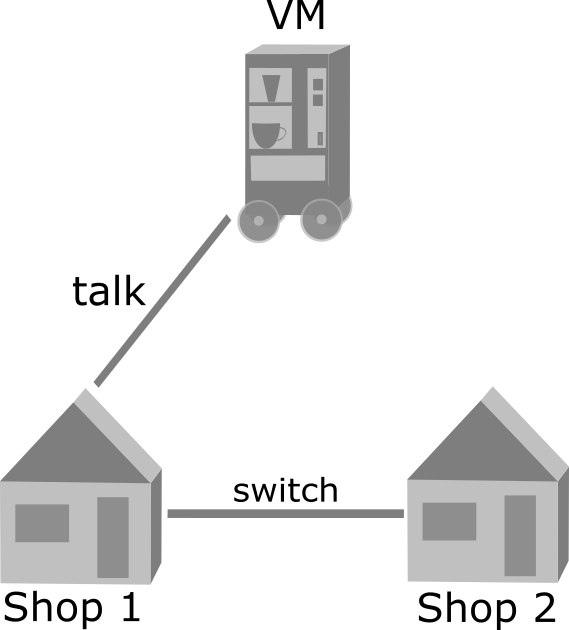
\includegraphics[width=0.45\textwidth]{./images/preliminaries/oz/oz_mobile_vending_machine_and_shops1.png}}}%
\hfill
\subcaptionbox{After switch}{\fbox{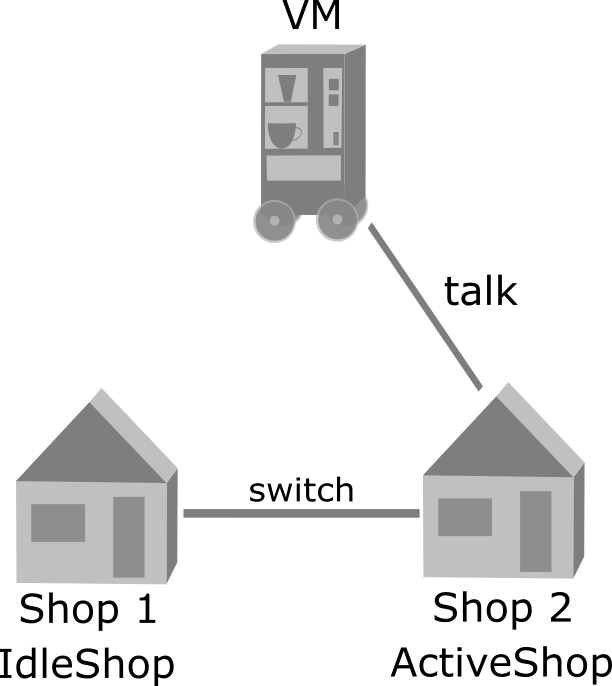
\includegraphics[width=0.45\textwidth]{./images/preliminaries/oz/oz_mobile_vending_machine_and_shops2.png}}}%
\caption{Mobile vending machine and shops}
\label{fig_oz_mobile_vending_machine_and_shops}%
\end{figure}

\begin{figure}[H]
\centering
\begin{sidebyside}
\begin{class}{ActiveShop(id: \integer)}
\\
\begin{state}
self, vmId, message: \integer
\\transferableOperation: nil | talk
\end{state} 
\\
\begin{init}
\\self = id
\\transferableOperation = talk
\end{init} 
\\
\begin{op}{switch\_\_\_\_\ then\ IdleShop}
x!: nil | talk
\ST
x! = transferableOperation
\\transferableOperation' = nil
\end{op}
\\
\begin{op}{talk}
\Delta (vmId, message)
\\y?, z?: \integer
\ST
y? = message'
\\z? = vmId'
\end{op}
\end{class}
\nextside
\begin{class}{IdleShop(id: \integer)}
\\
\begin{state}
self, vmId, message: \integer
\\transferableOperation: nil | talk
\end{state} 
\\
\begin{init}
\\self = id
\\transferableOperation = nil
\end{init} 
\\
\begin{op}{switch\_\_\_\_\ then\ ActiveShop}
\Delta (transferableOperation)
\\x?: nil | talk
\ST
x? = transferableOperation'
\end{op}
\end{class}
\end{sidebyside}
\caption{Active and idle shop.}
\label{fig_oz_active_idle_shop}
\end{figure}



\subsubsection{Restriction}
In this work when we use \oz{} to model an operation, we restrict our self to use only one type of parameters in the operation schema. Either input or output. This can be noticed in the operation schema $talk$ in:
\begin{itemize}
\item In \refFig{oz_vm_reference_name} all the parameters of the operation schema $talk$ are output paramaters.
\item In \refFig{fig_oz_unfixed_operation_schema_shop}  all the parameters of the operation schema $talk$ are input paramaters.
\end{itemize}
\textbf{Question:} why this restriction?\\
\textbf{Answer:} because a channel in \picalc{} is unidirectional pro reaction. In the next chapter we will map the \oz{} class constructs to  \picalc{} constructs, so we will map an \oz{} operation to an \picalc{} name , .i.e., channel. In \picalc{} a processes can send or receive over a channel pro reaction, but not the both together.
